\documentclass[UTF8]{ctexbook}
\usepackage{graphicx}
\usepackage{amsmath}

\title{桥梁大作业报告}
\author{组长:贺琪 \\ 组员:陈煜 \ 刘畅武 \ 杨昊光 \ 朱子霖}

\begin{document}
\maketitle 

\tableofcontents

%-------------------------这里是这个项目的整体描述---------------------------------
%----------------------------------------------------------------------------------
\newpage
\section{总述}
\subsection{项目描述}
桥模型由桥墩(pier),桥面(floor),支撑梁(support beam),河堤(river bank)和钢缆(cables)五部分组成,其中桥墩和河堤用实体单元建模,桥面用板单元建模,支撑梁用梁单元建模,钢缆用杆单元建模,如图1 所示。\\

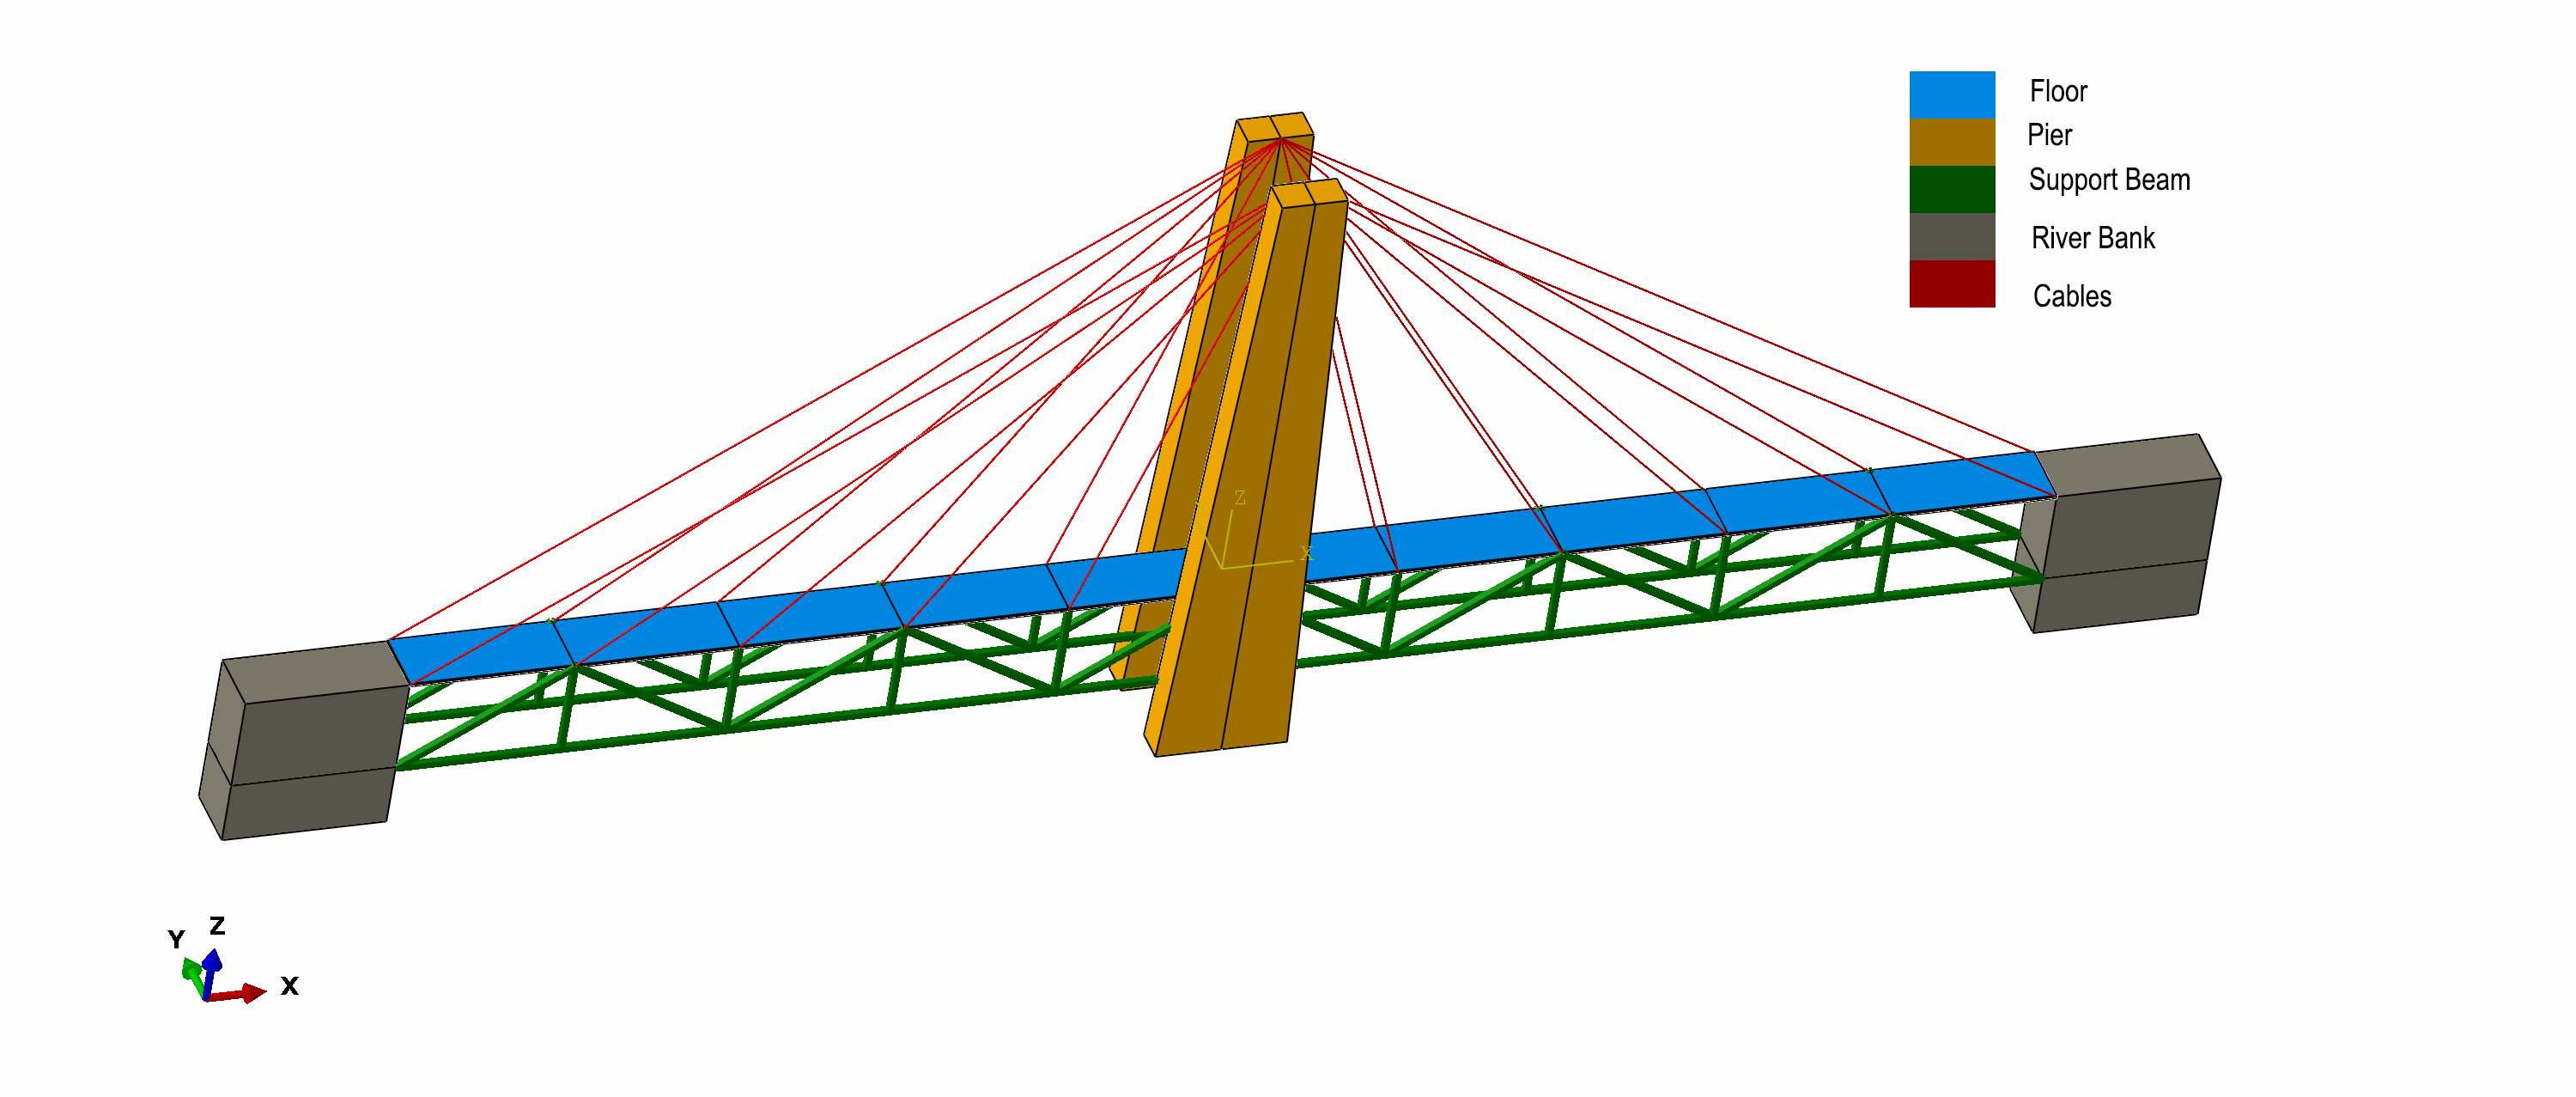
\includegraphics[width=\textwidth]{01.png} % Include the image placeholder.png

\textbf{桥墩}:

桥墩在XZ方向为左右对称梯形,如图2所示,梯形高200,上底为20,下底40,在y方向上厚度为10。桥面位于距桥墩底50处。两个桥墩顶面内侧中点为所有钢缆的与桥墩的连接点。(参照图1)

采用实体单元建模

\begin{center}
\begin{tabular}{ll}
材料&:Concrete\\
弹性模量&:25e9\\
泊松比&:0.3\\
密度&:2320\\
\end{tabular}
\end{center}


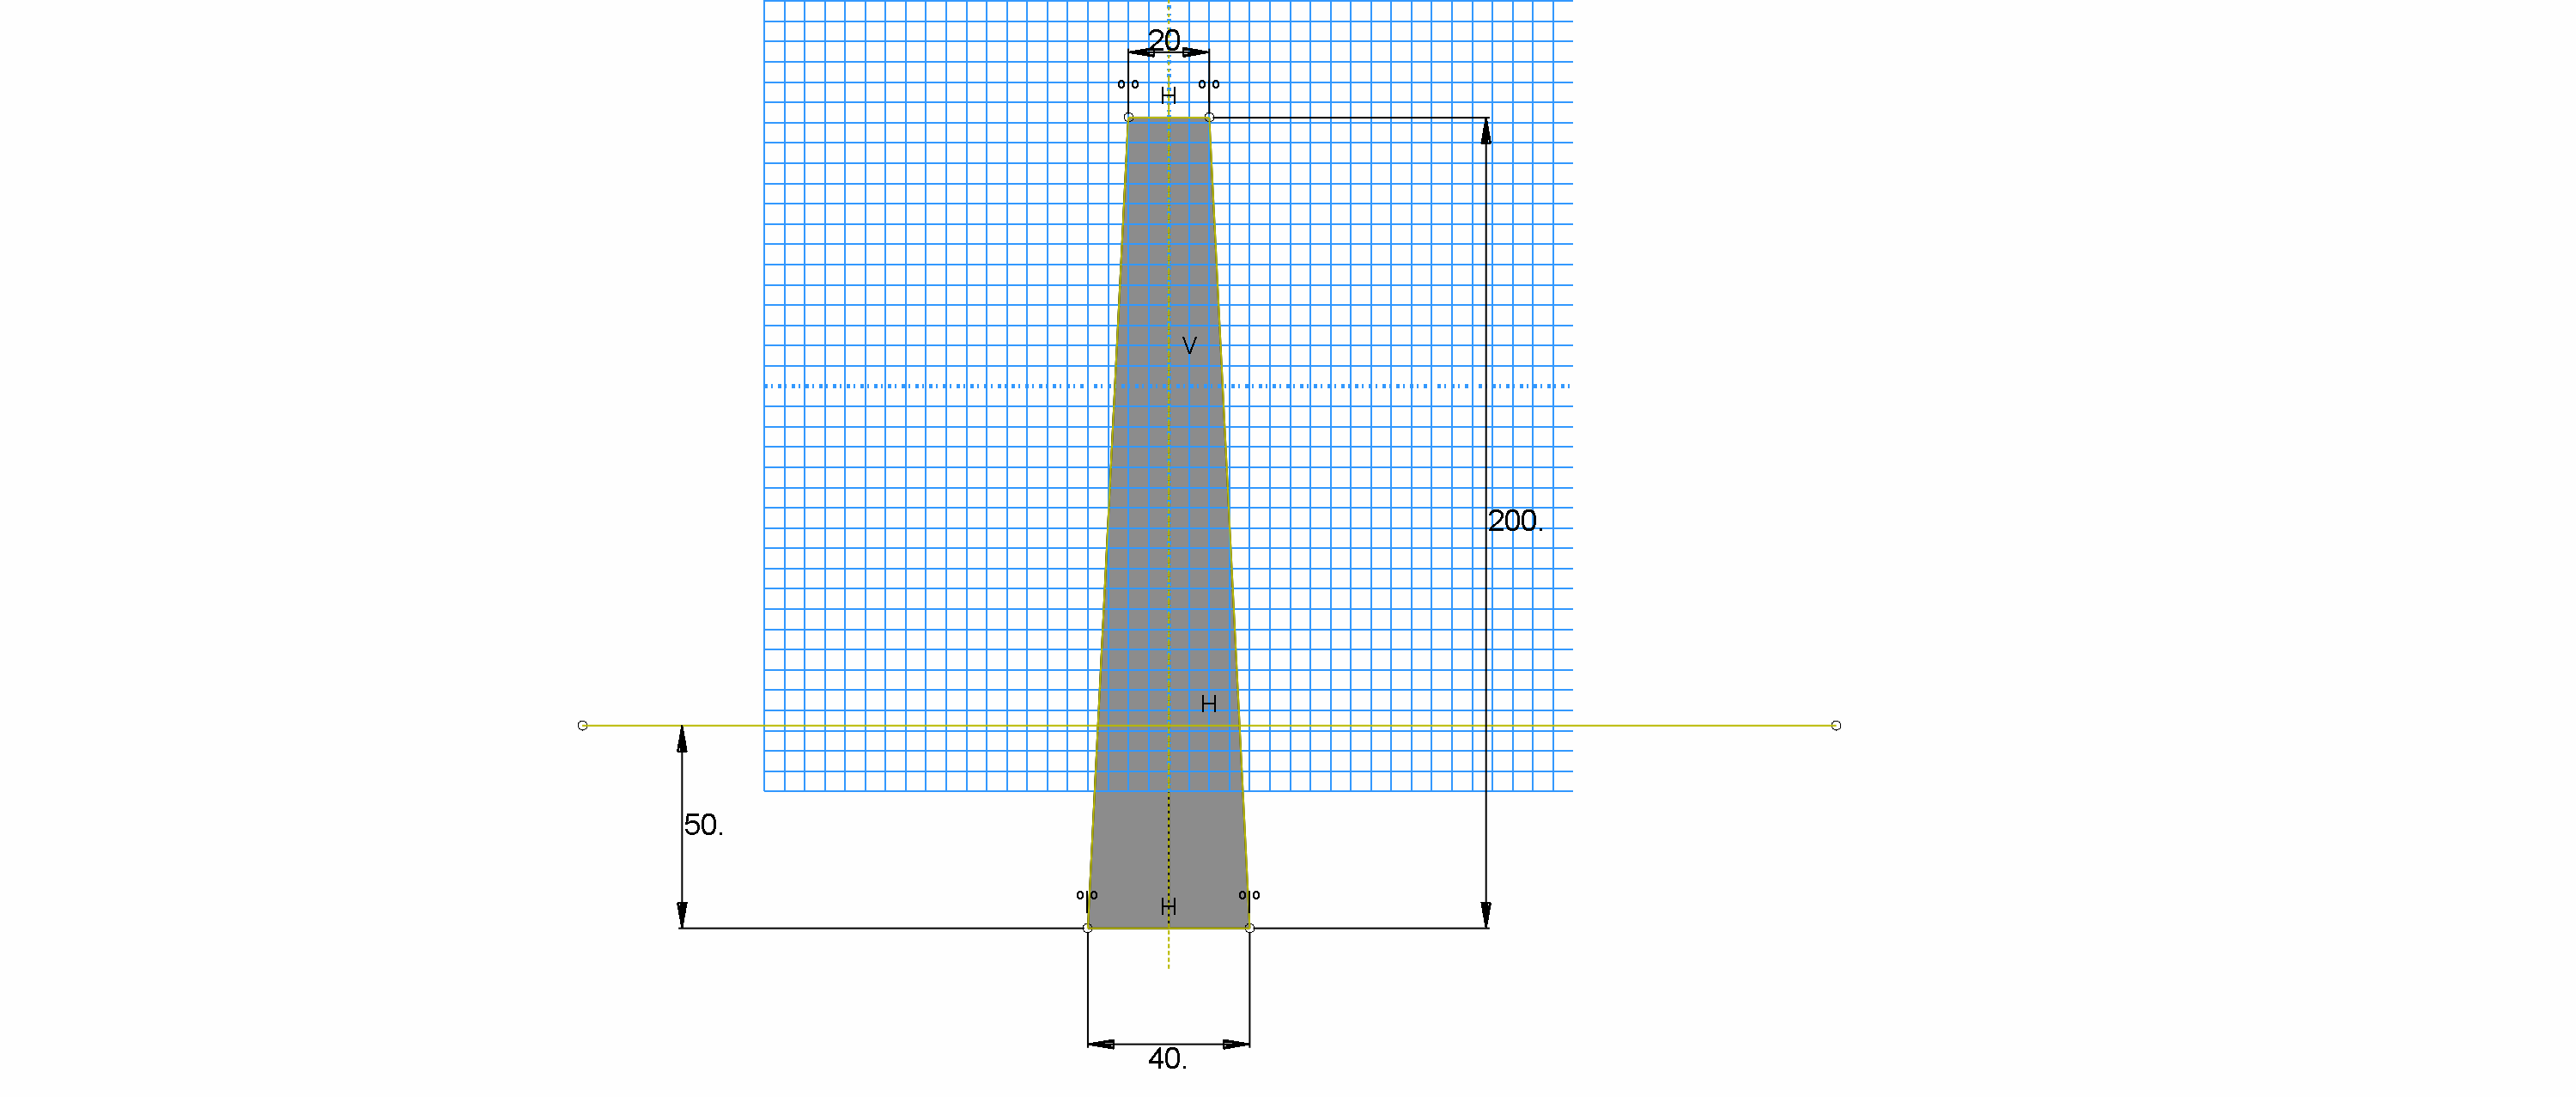
\includegraphics[width=\textwidth]{02.png}

\textbf{桥面}:

桥面位于z=0的平面内,如图3所示,为长方形,长为500,宽为20,厚度为1。在桥面上下边对称地布置钢缆连接点,每个钢缆连接点相距50,共计2×2×5=20个钢缆连接点。每根钢缆另一端连接桥墩顶面内侧中点。(参照图1)

采用板单元建模

\begin{center}
\begin{tabular}{ll}
材料&:Concrete\\
弹性模量&:25e9\\
泊松比&:0.3\\
密度&:2320\\
\end{tabular}
\end{center}

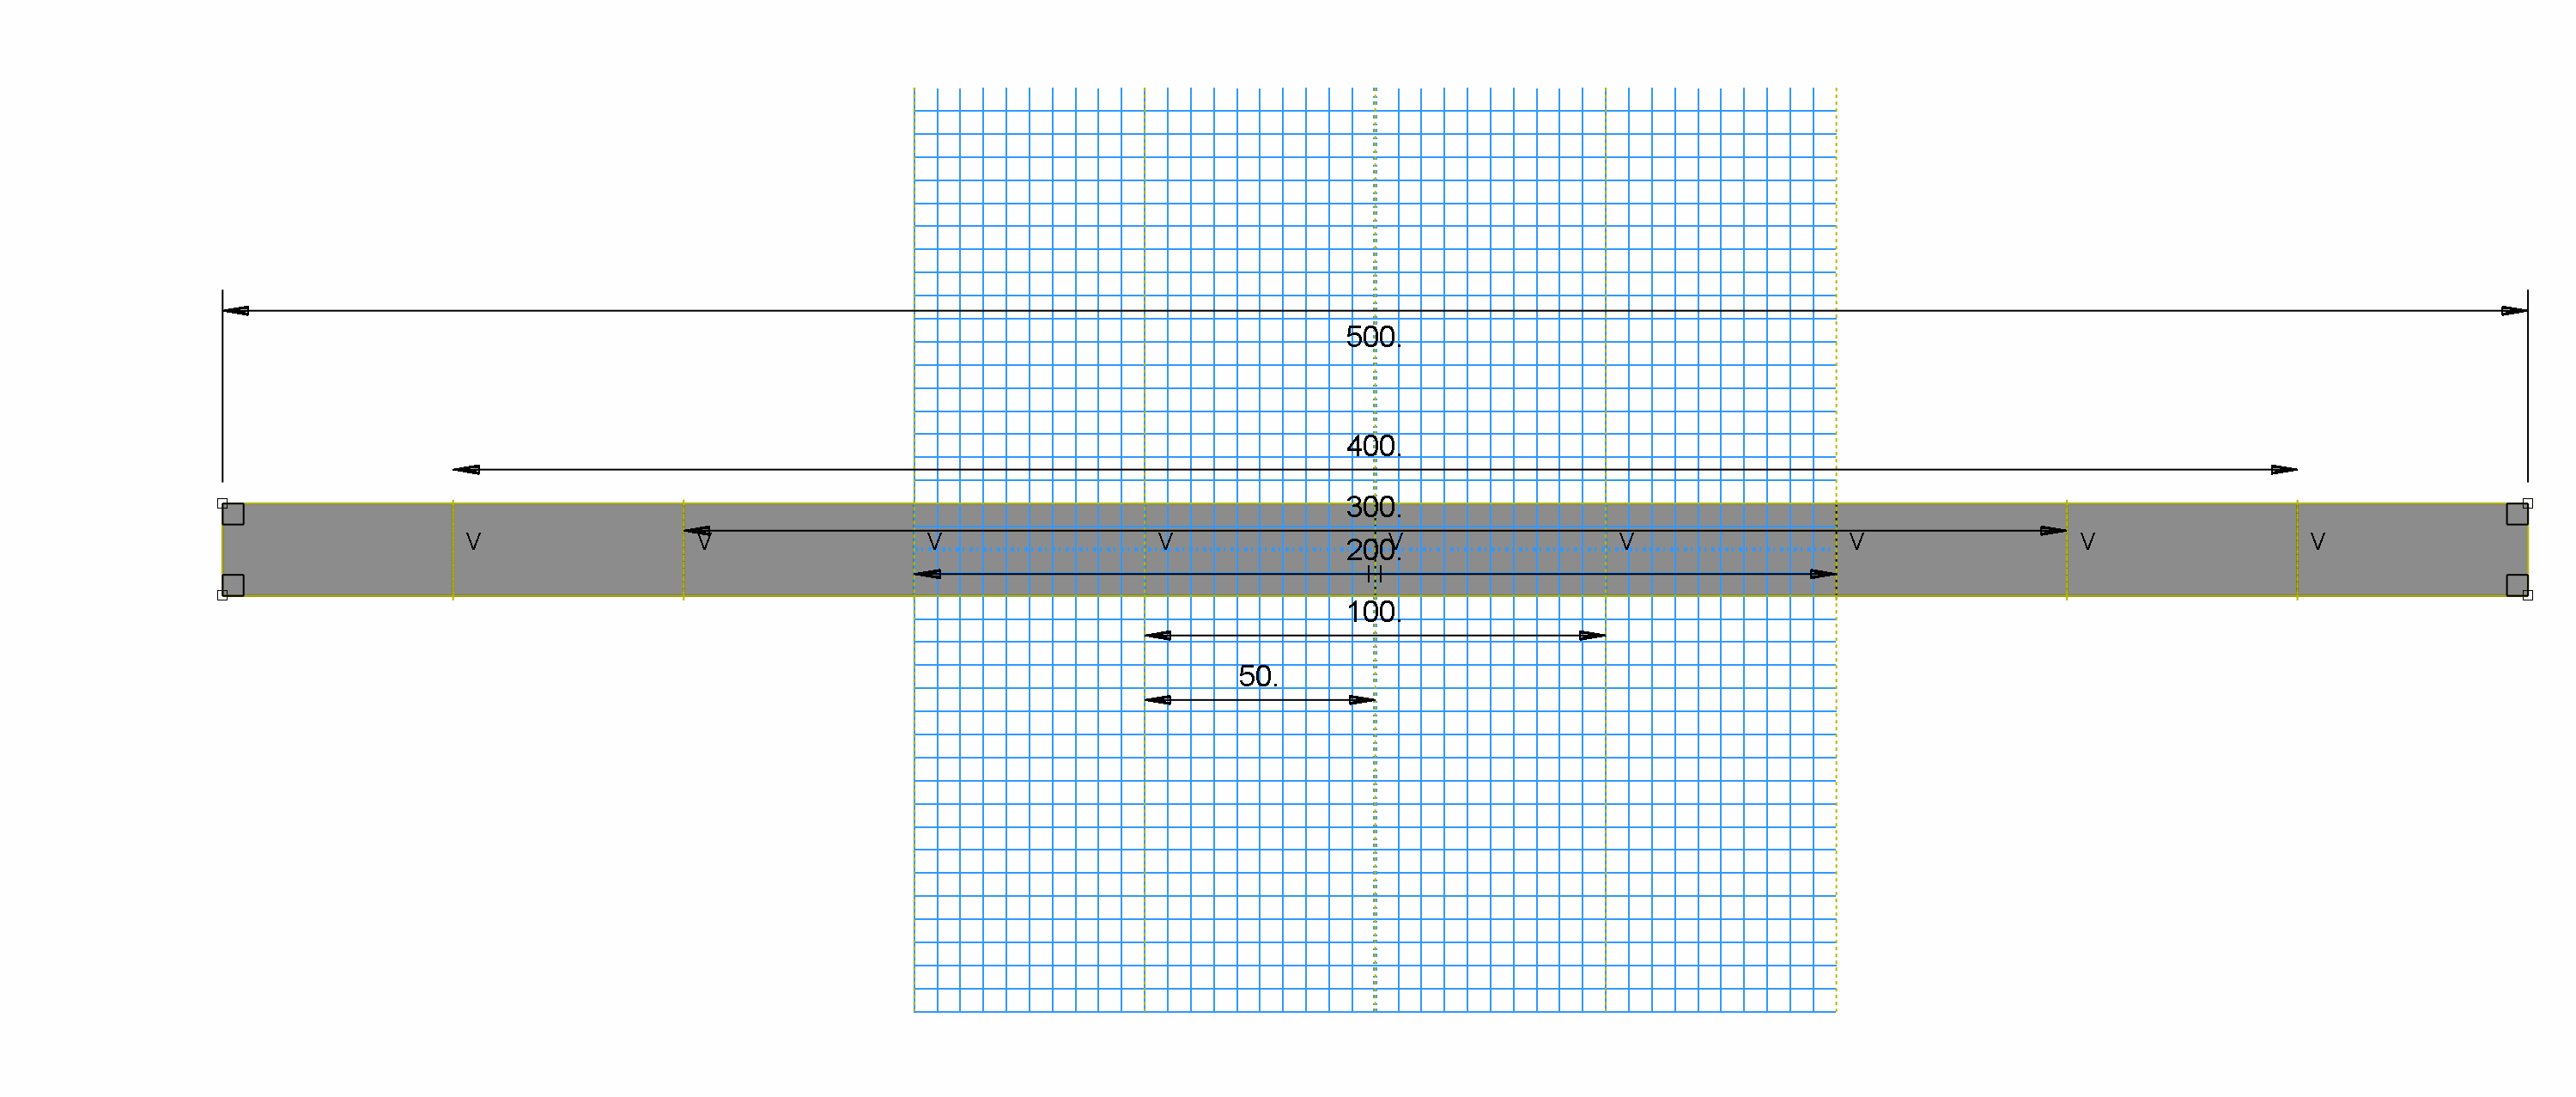
\includegraphics[width=\textwidth]{03.png}

\textbf{河堤}:

河堤为50×50×20的立方体,如图1所示,变长为20的一边与桥面相铰接,另外在距离底面20处与支撑梁相铰接。(铰接指对应结点平动自由度相同,转动自由度自由)

采用实体单元建模。

\begin{center}
\begin{tabular}{ll}
材料&:Granite\\
弹性模量&:60e9\\
泊松比&:0.27\\
密度&:2770\\
\end{tabular}
\end{center}

\textbf{支撑梁}:

支撑梁共有两组,分别位于桥面两侧下方,其结构左右对称,如图4所示。支撑梁上部每个结点与桥面相铰接,两组共计2×9=18个结点。两端结点与河堤相铰接,共计2×2=4个结点。

采用梁单元建模,梁截面为正方形筒,边长为2,厚度为0.1。

\begin{center}
\begin{tabular}{ll}
材料&:Aluminum\\
弹性模量&:70e9\\
泊松比&:0.346\\
密度&:2710\\
\end{tabular}
\end{center}

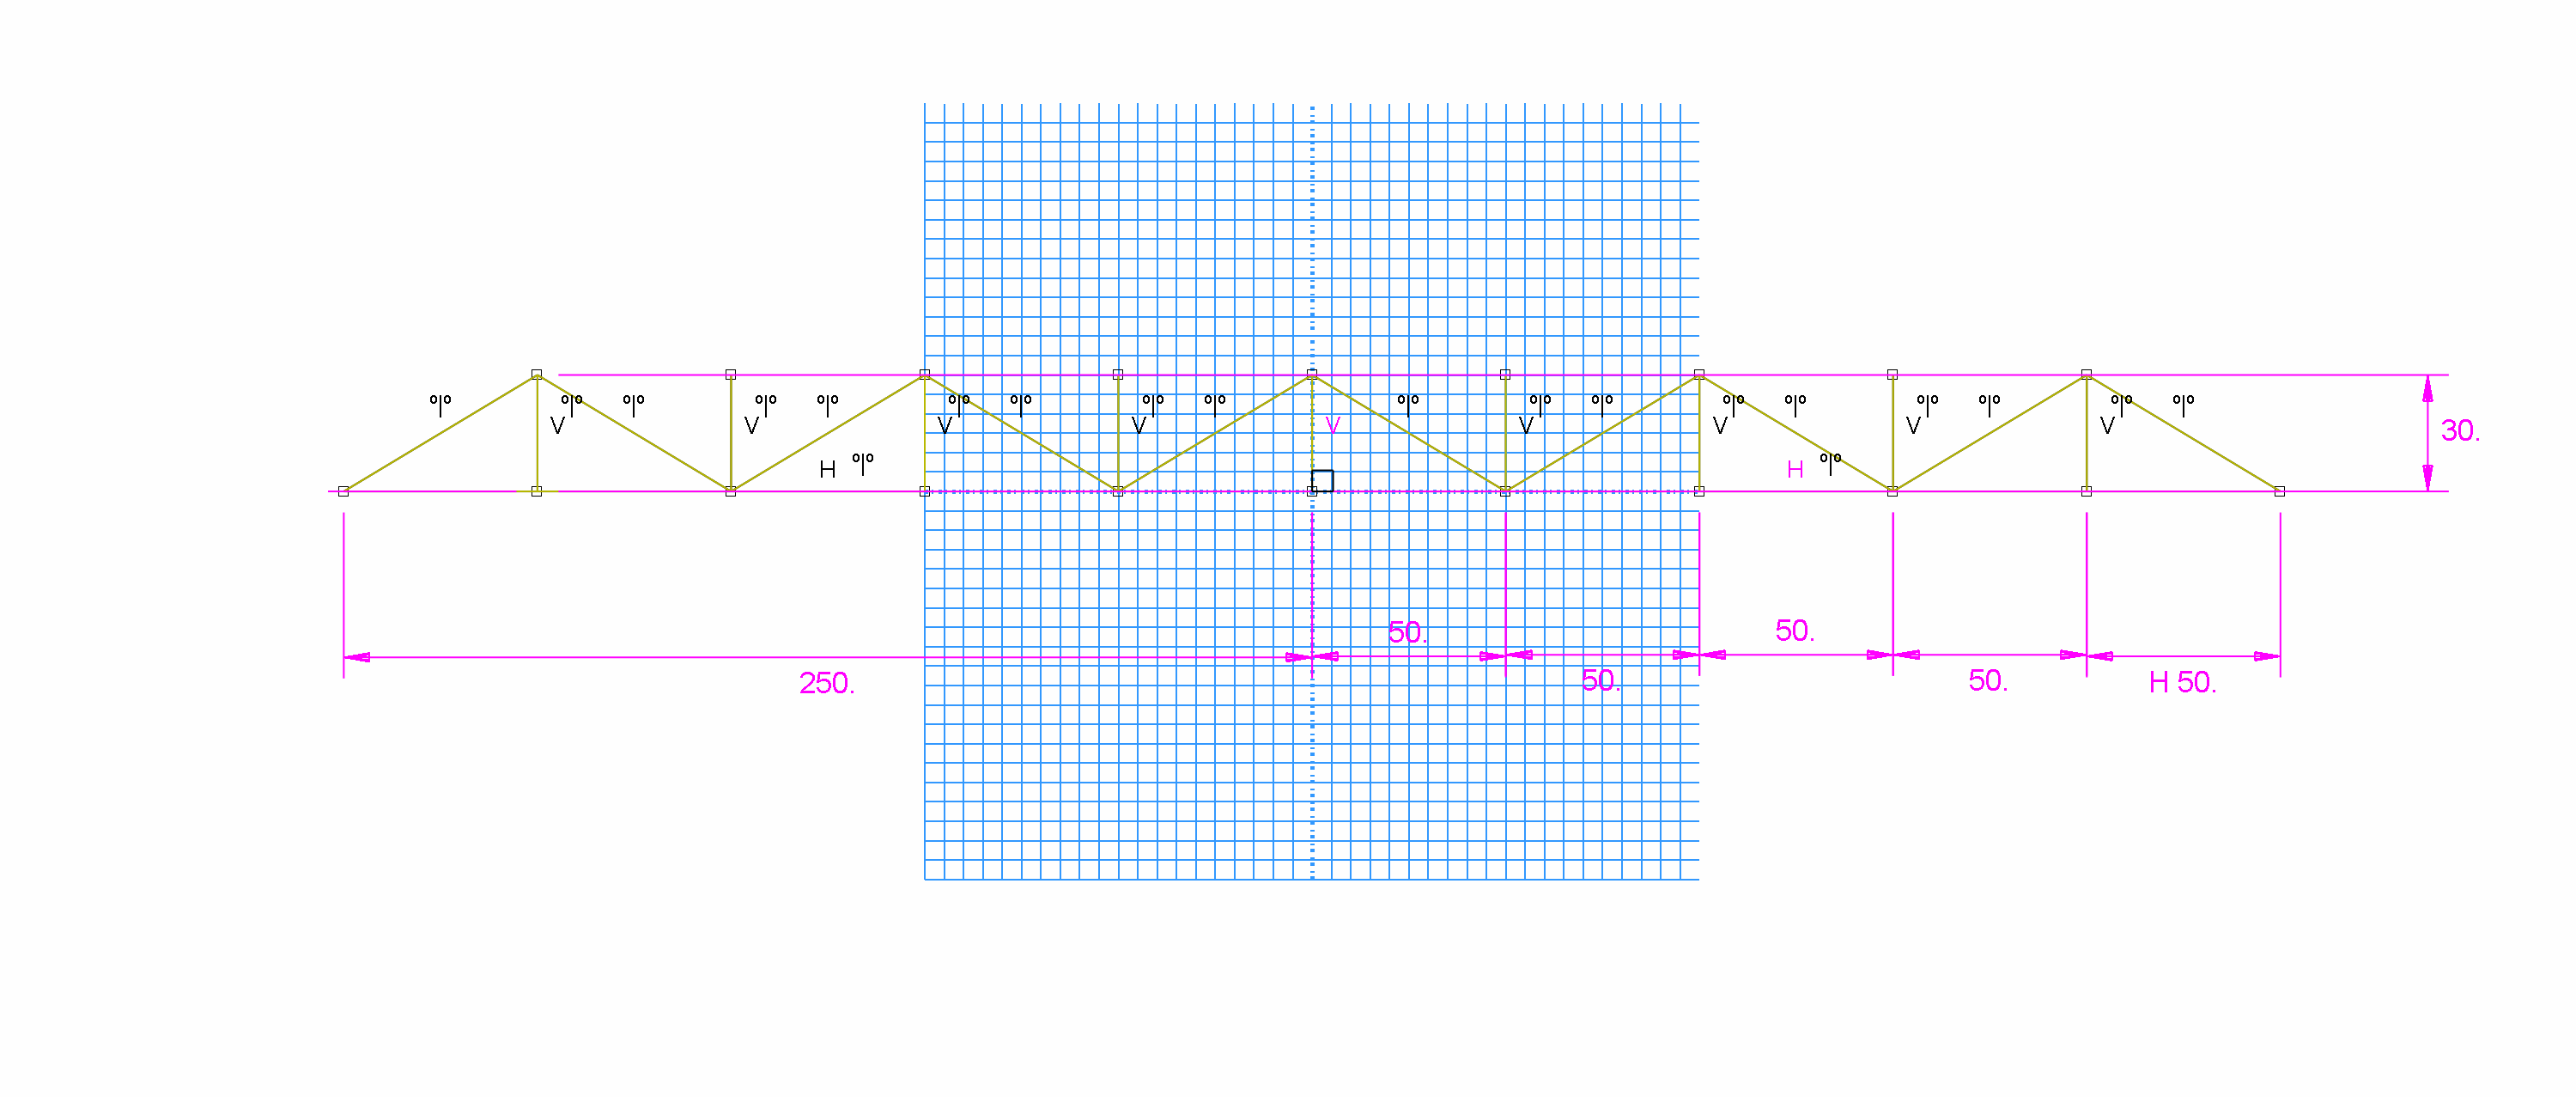
\includegraphics[width=\textwidth]{04.png}

\textbf{钢缆}:

连接桥面与桥墩,共计2×2×5=20根。每根截面积为0.25。

采用杆单元建模

\begin{center}
\begin{tabular}{ll}
材料&:Steel\\
弹性模量&:117e9\\
泊松比&:0.266\\
密度&:7860\\
\end{tabular}
\end{center}

\subsection{Abaqus结果}
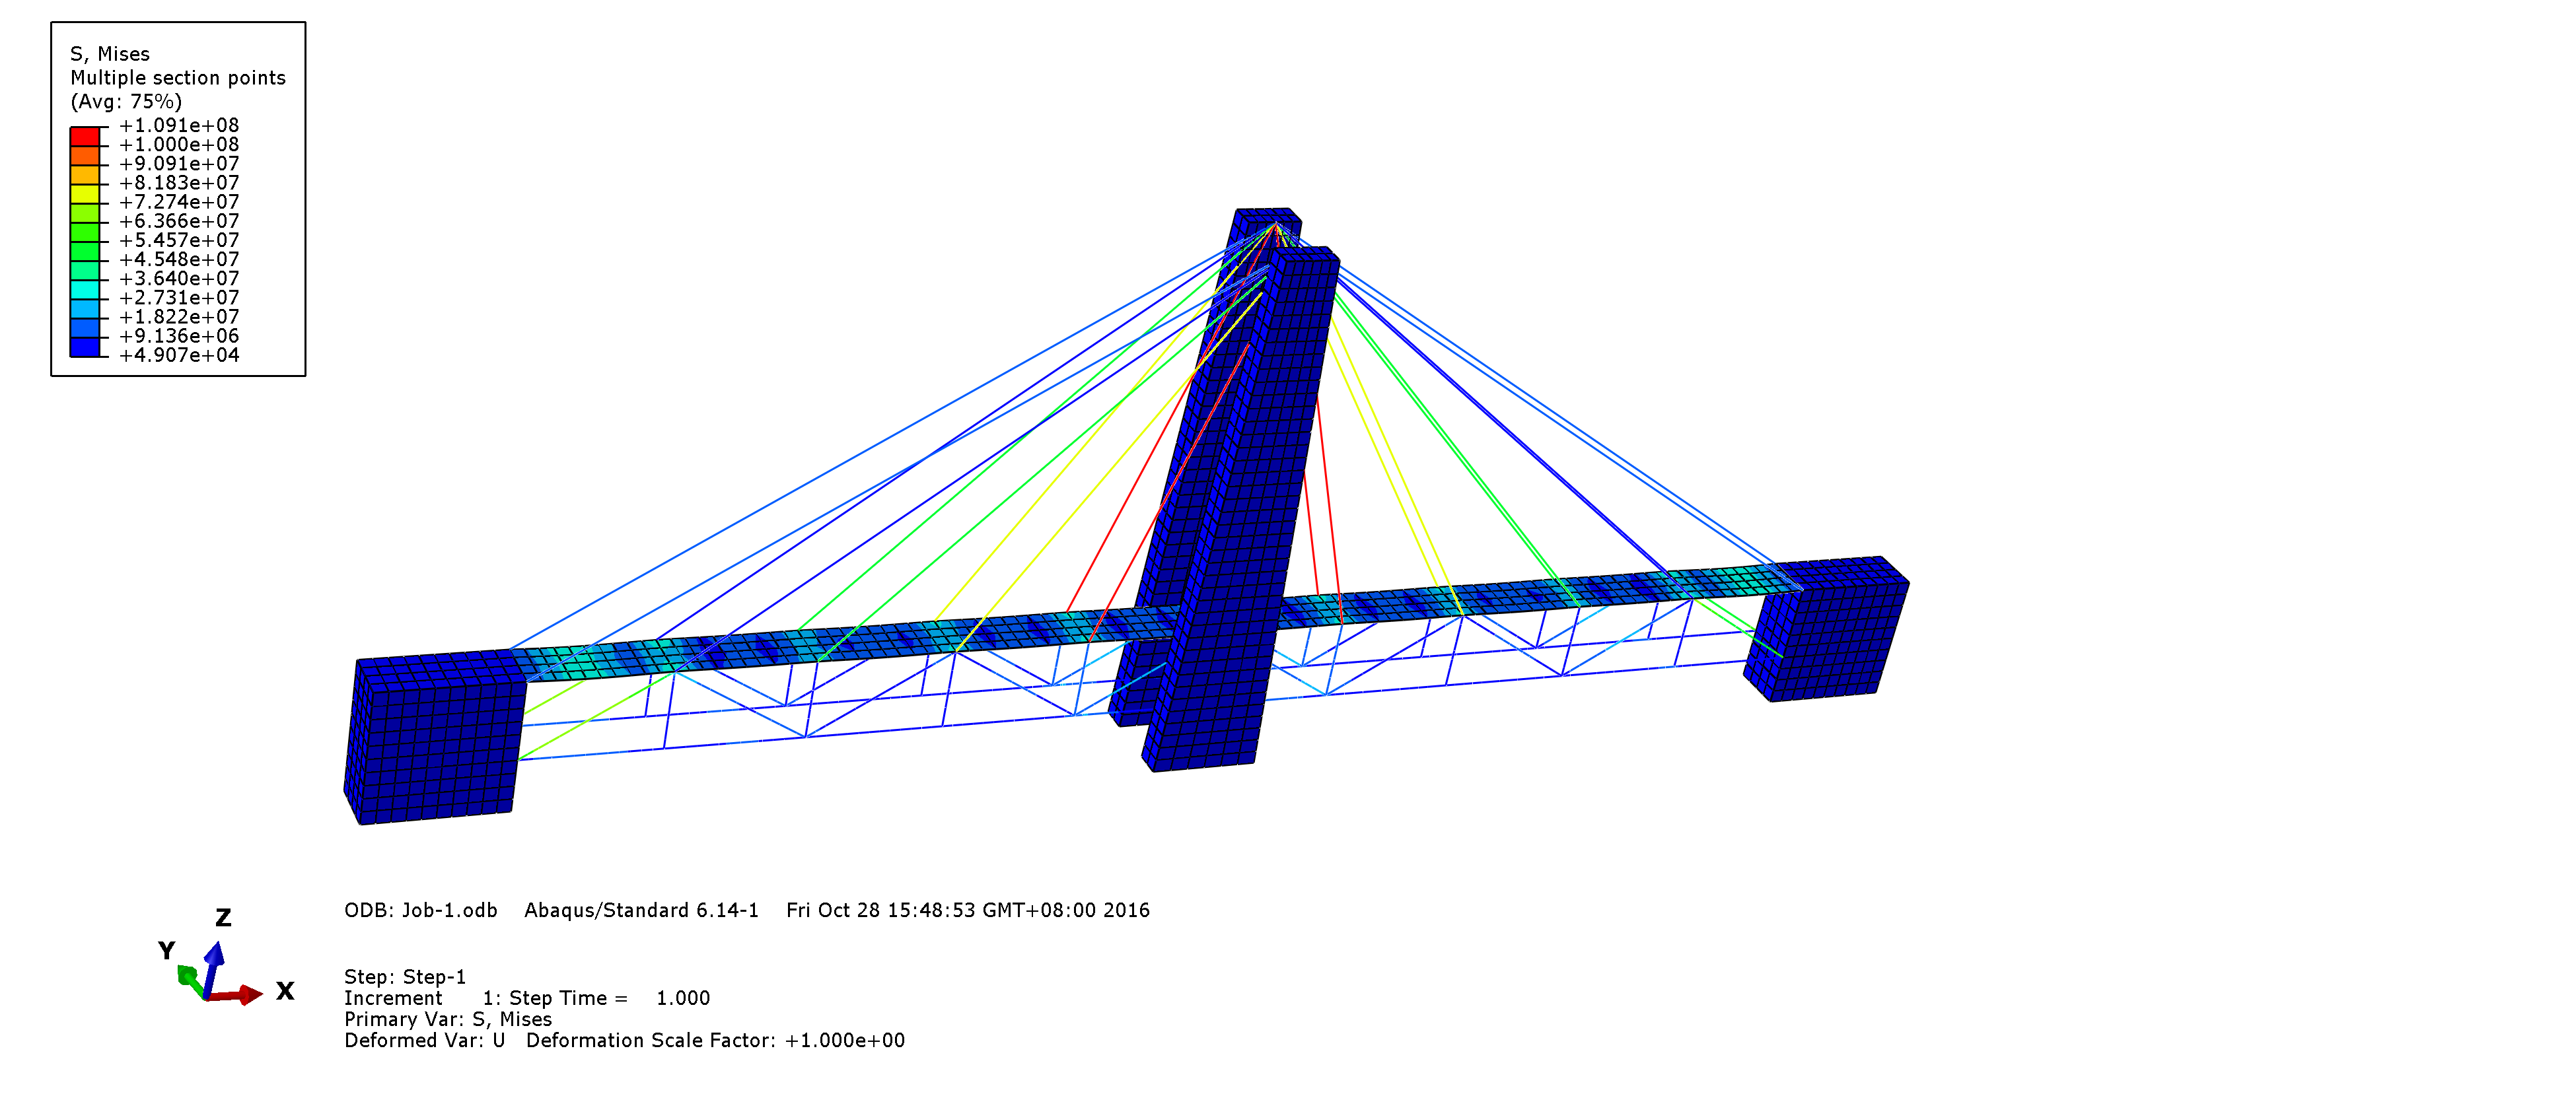
\includegraphics[width=\textwidth]{05.png}


%-------------------------这里是各个部分的描述-------------------------------------
%----------------------------------------------------------------------------------
\section{桥梁功能实现方案}
\subsection{前处理}

\subsection{SPR}

\subsection{后处理}

\subsection{8H}

\subsection{Beam}

\subsection{Shell}

\subsection{半带宽优化}

\subsection{稀疏存储求解器}

%-------------------------这里是其他单元的描述-------------------------------------
%----------------------------------------------------------------------------------
\section{其他单元}
\subsection{3T}

\subsection{4Q}

\subsection{6T}

\subsection{8Q}

\subsection{9Q}

\subsection{4T}

\subsection{铁木辛柯梁}

\subsection{Plate}

\subsection{无限单元}

\subsection{超级单元}

\subsection{过渡单元}

%-------------------------这里是其他功能的描述-------------------------------------
%----------------------------------------------------------------------------------
\section{高级功能}
\subsection{弹塑性杆分析}

\subsection{模态分析}

\subsection{动力学响应分析}

\end{document}